% --- CORRESPONDE A: casos.tex ---
% --- DIAPOSITIVA 14: CASOS DE ESTUDIO Y CONJETURAS ---\

% --- NUEVA DIAPOSITIVA: MARCO TEÓRICO - OBJETIVOS DEL CAPÍTULO 2 ---
\begin{frame}{Marco Teórico: Objetivos del Capítulo 2}
	\begin{block}{Contenido del Capítulo 2} \footnotesize
		En el Capítulo 2 se establecieron los cimientos teóricos que guiarán todo el trabajo:
		\begin{itemize}
			\item Se revisaron las nociones básicas de polinomios ortogonales y sus matrices de momentos
			\item Se introdujo el operador de multiplicación $\mathcal{D}$ y se formalizó la ortogonalidad de Sobolev junto con el problema central de la localización de ceros
			\item Además, se contextualizó el estado del arte resaltando la utilidad de la aproximación matricial y de los estudios numéricos para la teoría de los ceros bajo diferentes productos internos
		\end{itemize}

		El objetivo de este segundo capítulo es \textbf{aplicar} aquel armazón teórico a los 4 casos concretos y, a partir de la evidencia obtenida, \textbf{formular conjeturas} que orienten futuras demostraciones rigurosas. El capítulo se organiza en tres secciones principales:
	\end{block}
\end{frame}

% --- NUEVA DIAPOSITIVA: MARCO TEÓRICO - SECCIONES DEL CAPÍTULO 2 ---
\begin{frame}{Marco Teórico: Secciones del Capítulo 2}
	\begin{block}{Organización en Tres Secciones} \footnotesize
		\begin{itemize}
			\item \textbf{3.1 Caso real} - Se analizan productos de Sobolev definidos sobre soportes en la recta real. La simplicidad geométrica permite contrastar los resultados con referencias clásicas y calibrar las herramientas algebraicas presentadas anteriormente.

			\item \textbf{3.2 Caso circunferencia} - El estudio se traslada al plano complejo considerando medidas soportadas en circunferencias. Esta configuración pone de relieve la influencia de transformaciones de semejanza y la interacción entre la topología del soporte y la distribución de ceros.

			\item \textbf{3.3 Análisis y conjeturas} - Reúne las observaciones extraídas de ambos escenarios para proponer conjeturas sobre:
			      \begin{enumerate}
				      \item Cotas uniformes para los ceros en función del radio o de la posición relativa de los soportes
				      \item El comportamiento asintótico de valores singulares sucesivos de las secciones $\mathbf{D}_n$ y su relación con el radio espectral
				      \item La influencia de la dominación secuencial o matricial en la acotación de $\mathcal{D}$
			      \end{enumerate}
		\end{itemize}
	\end{block}
\end{frame}

\begin{frame}{Casos de Estudio y Conjeturas}
	\footnotesize % Ajustar tamaño de fuente si es necesario
	A continuación, se presentan ejemplos numéricos para ilustrar el comportamiento de los ceros y los parámetros espectrales en diferentes escenarios. Estos ejemplos motivarán las conjetas clave del trabajo.

	\textbf{Metodología de Visualización:}
	Para cada ejemplo, se muestra:
	\begin{itemize}
		\item Ceros de $\varphi_n$ para un $n$ fijo (cero de mayor módulo en rojo).
		\item Todos los ceros $\{\varphi_i\}_{i=0}^n$ (radios espectrales en rojo).
		\item Evolución de $\rho(\mathbf{D}_n)$ (círculos), $\sigma_{1,n}$ (diamantes), $\sigma_{2,n}$ (cuadrados).
		\item Datos espectrales relevantes.
	\end{itemize}
\end{frame}

% --- DIAPOSITIVA 15A: CASO REAL - EJEMPLO SECUENCIALMENTE DOMINADO ---
\begin{frame}{Caso Real: Ejemplo Secuencialmente Dominado}
	\textbf{Ejemplo 1:}\;
	$\displaystyle
		\langle p,q\rangle_S
		=\int_{-2}^{2} p(t)q(t) \, dt
		+ \int_{-1}^{1} p'(t)q'(t) \, dt$
	\vspace{-0.8em} % Ajustado vspace
	\begin{figure}
		\begin{subfigure}[b]{0.4\columnwidth} % Modificado
			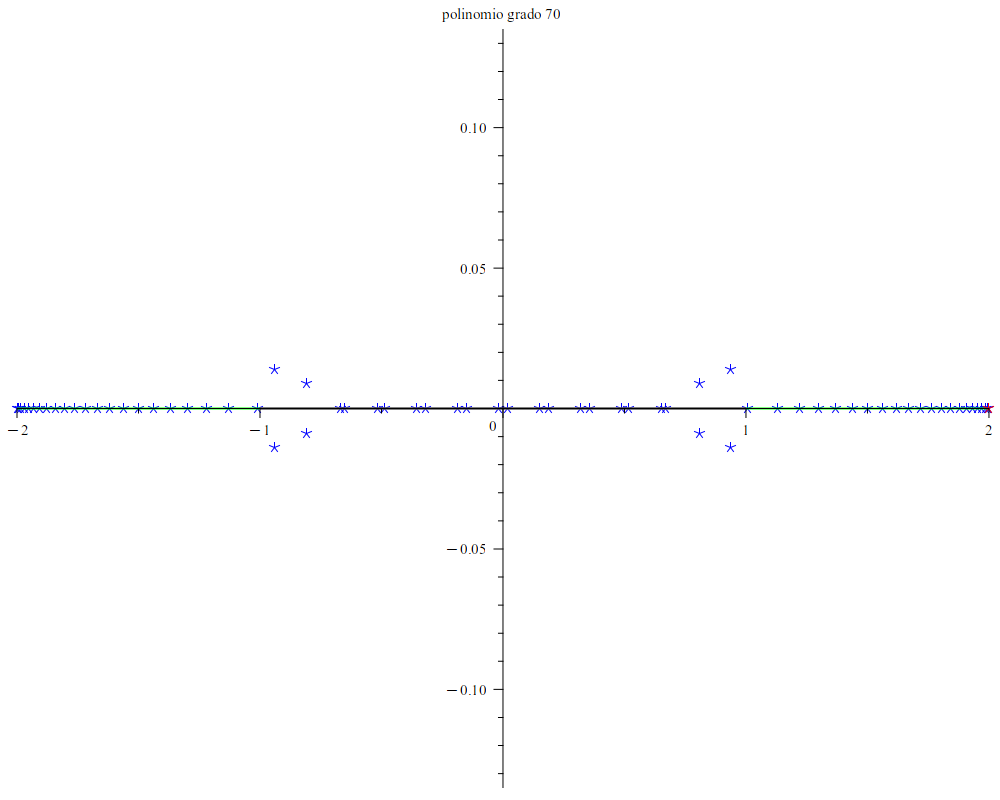
\includegraphics[width=\linewidth]{tfg_latex_etsiinf-2023.02.20/include/a-2b2c1d-1_zero.png}
			\caption*{\scriptsize Ceros $\varphi_{70}$}
		\end{subfigure}\hfill
		\begin{subfigure}[b]{0.4\columnwidth} % Modificado
			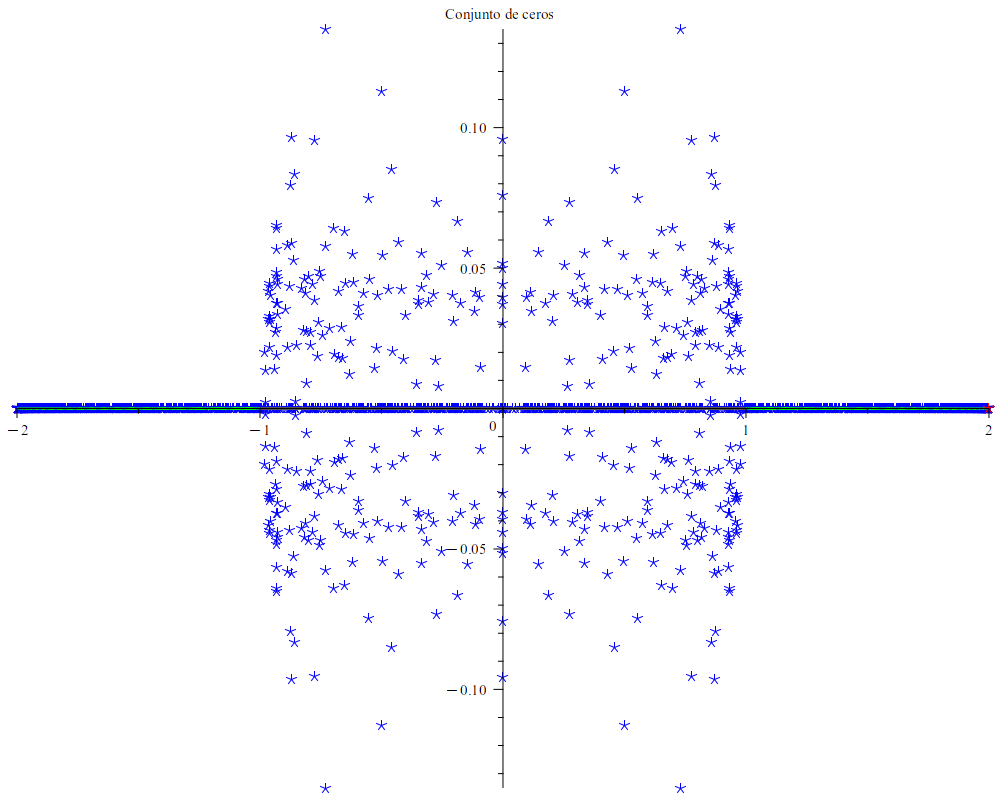
\includegraphics[width=\linewidth]{tfg_latex_etsiinf-2023.02.20/include/a-2b2c1d-1_zeros.png}
			\caption*{\scriptsize Ceros $\varphi_{0},\dots,\varphi_{70}$}
		\end{subfigure}
		\vspace{-0.5em} % Ajustado vspace, modificado de -0.3em
		\begin{subfigure}[b]{0.4\columnwidth} % Modificado
			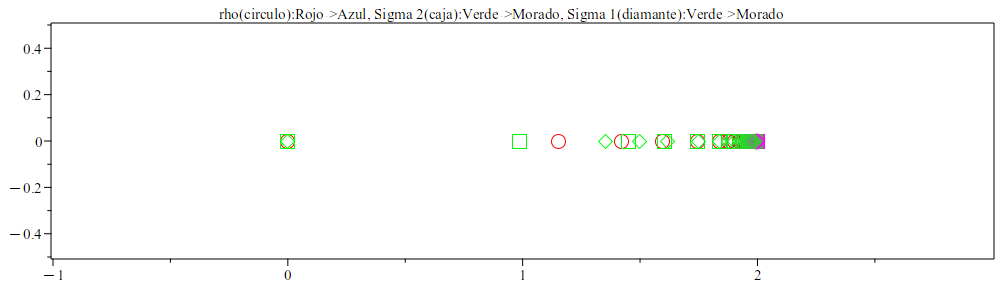
\includegraphics[width=\linewidth]{tfg_latex_etsiinf-2023.02.20/include/a-2b2c1d-1.png}
			\caption*{\scriptsize Sec. espectral}
		\end{subfigure}\hfill
		\begin{subfigure}[b]{0.4\columnwidth} % Modificado
			\tiny
			\textbf{Datos ($n=70$):}
			\begin{itemize}
				\item $\sigma_{1,70}=1.999$
				\item $\sigma_{2,70}=1.999$
				\item $R = 2$
				\item $\rho(\mathbf{D}_{70})=1.999$
				\item $\max\rho_k=1.999$
			\end{itemize}
		\end{subfigure}
	\end{figure}
	\vspace{-1em} % Ajustado vspace
\end{frame}

% --- DIAPOSITIVA 15B: CASO REAL - EJEMPLO SECUENCIALMENTE DOMINADO (OBSERVACIONES) ---
\begin{frame}{Caso Real: Ejemplo Secuencialmente Dominado - Observaciones}
	\begin{block}{Observaciones (Ej.1)} \small
		Caso secuencialmente dominado. $\mathcal{D}$ acotado. $\sigma_{1,n}, \sigma_{2,n}, \rho(\mathbf{D}_n) \to R=2$. Ceros en $[-2,2]$.
	\end{block}
\end{frame}

% --- DIAPOSITIVA 16A: CASO REAL - EJEMPLO SOPORTES DISJUNTOS ---
\begin{frame}{Caso Real: Ejemplo Soportes Disjuntos}
	\textbf{Ejemplo 2:}\;
	$\displaystyle
		\langle p, q \rangle_S
		= \int_{0}^{10} p(t)q(t) \, dt
		+ \int_{30}^{40} p'(t)q'(t) \, dt$
	\vspace{-0.8em}
	\begin{figure}
		\begin{subfigure}[b]{0.4\columnwidth} % Modificado
			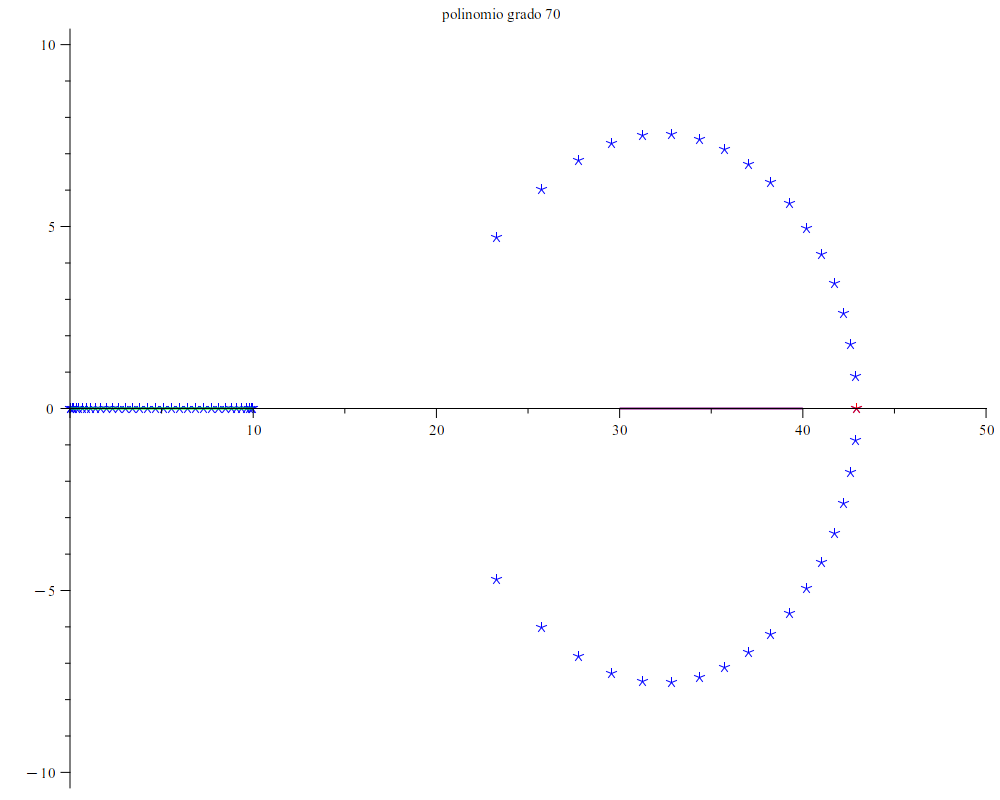
\includegraphics[width=\linewidth]{tfg_latex_etsiinf-2023.02.20/include/a0b10c30d40_zero.png}
			\caption*{\scriptsize Ceros $\varphi_{70}$}
		\end{subfigure}\hfill
		\begin{subfigure}[b]{0.4\columnwidth} % Modificado
			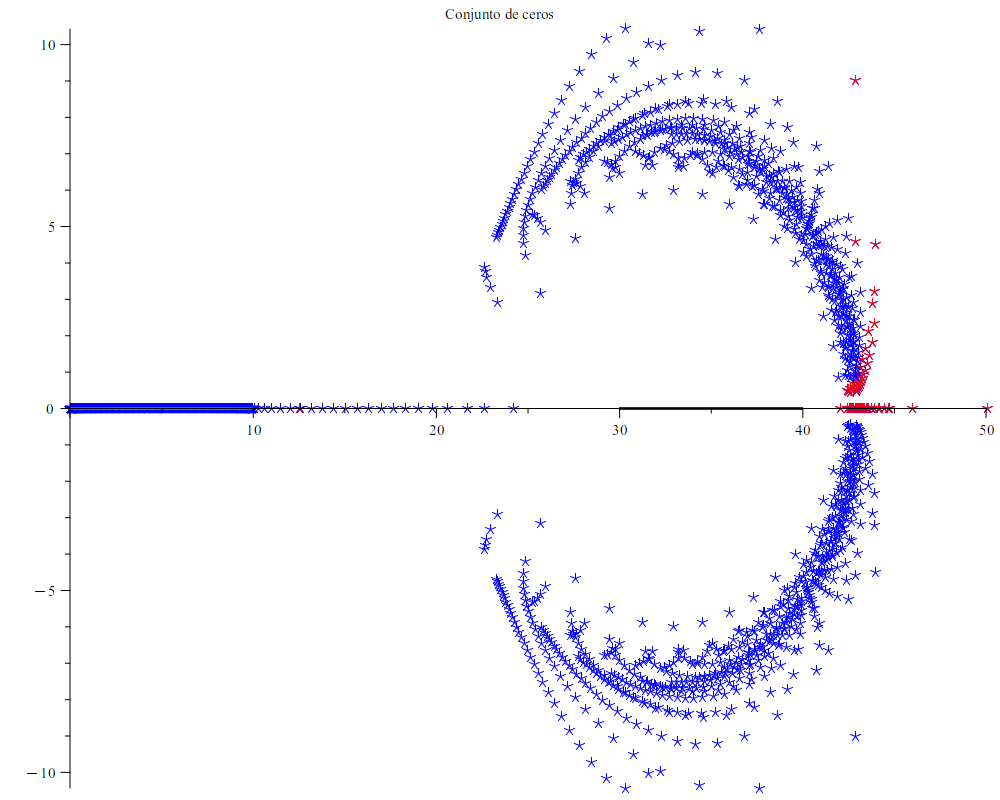
\includegraphics[width=\linewidth]{tfg_latex_etsiinf-2023.02.20/include/a0b10c30d40_zeros.png}
			\caption*{\scriptsize Ceros $\varphi_{0},\dots,\varphi_{70}$}
		\end{subfigure}
		\vspace{-0.5em} % Modificado de -0.3em
		\begin{subfigure}[b]{0.4\columnwidth} % Modificado
			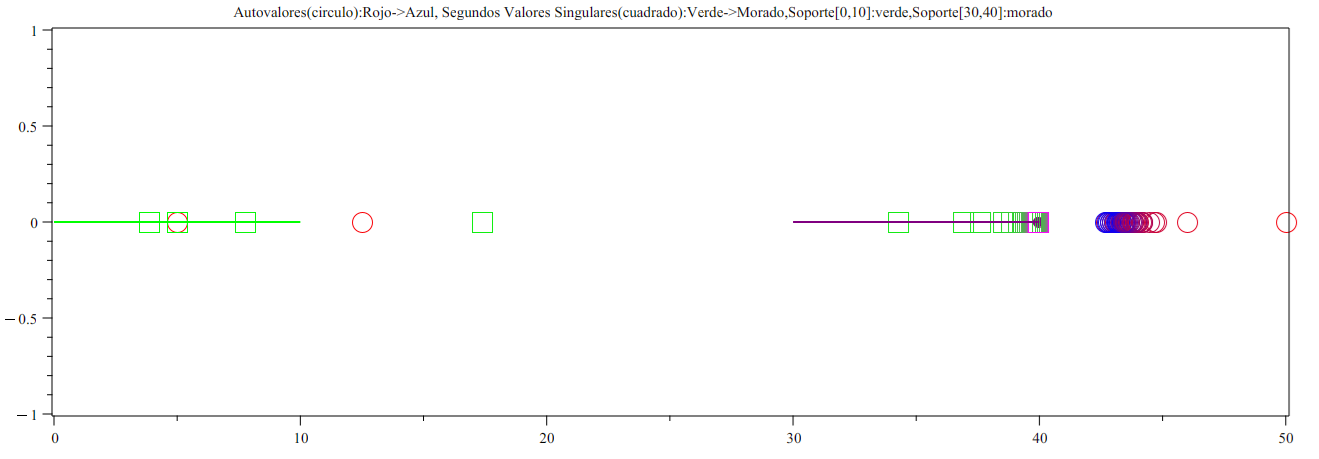
\includegraphics[width=\linewidth]{tfg_latex_etsiinf-2023.02.20/include/a0b10c30d40.png}
			\caption*{\scriptsize Sec. espectral}
		\end{subfigure}\hfill
		\begin{subfigure}[b]{0.4\columnwidth} % Modificado
			\tiny
			\textbf{Datos ($n=70$):}
			\begin{itemize}
				\item $\sigma_{1,70} \approx 9.27\text{e}16$
				\item $\sigma_{2,70} \approx 39.998$
				\item $R = 40$
				\item $\rho(\mathbf{D}_{70}) \approx 42.930$
				\item $\max\rho_k \approx 50.052$
			\end{itemize}
		\end{subfigure}
	\end{figure}
	\vspace{-1em}
\end{frame}

% --- DIAPOSITIVA 16A.1: CASO REAL - EJEMPLO SOPORTES DISJUNTOS (GRÁFICOS DE CEROS) ---
\begin{frame}{Caso Real: Ejemplo Soportes Disjuntos (Gráficos de Ceros)}
	\textbf{Ejemplo 2:}\;
	$\displaystyle
		\langle p, q \rangle_S
		= \int_{0}^{10} p(t)q(t) \, dt
		+ \int_{30}^{40} p'(t)q'(t) \, dt$
	\vspace{-0.8em}
	\begin{figure}
		\begin{subfigure}[b]{0.4\columnwidth} % Modificado
			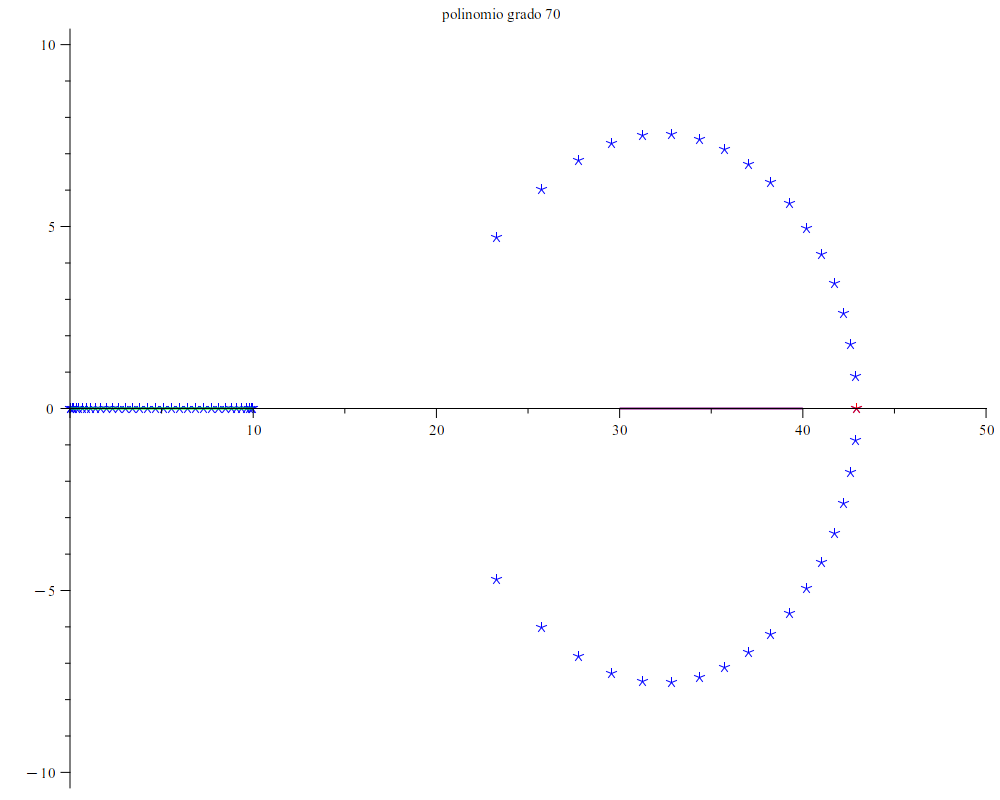
\includegraphics[width=\linewidth]{tfg_latex_etsiinf-2023.02.20/include/a0b10c30d40_zero.png}
			\caption*{\scriptsize Ceros $\varphi_{70}$}
		\end{subfigure}\hfill
		\begin{subfigure}[b]{0.4\columnwidth} % Modificado
			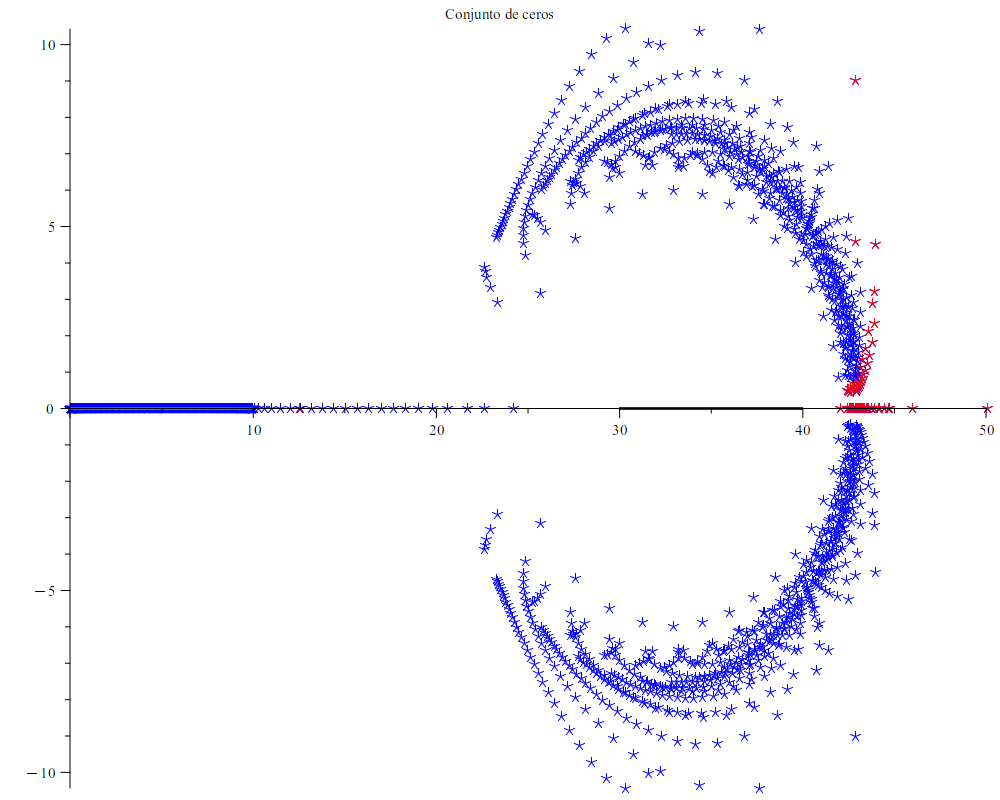
\includegraphics[width=\linewidth]{tfg_latex_etsiinf-2023.02.20/include/a0b10c30d40_zeros.png}
			\caption*{\scriptsize Ceros $\varphi_{0},\dots,\varphi_{70}$}
		\end{subfigure}
	\end{figure}
	\vspace{-1em}
\end{frame}

% --- DIAPOSITIVA 16A.2: CASO REAL - EJEMPLO SOPORTES DISJUNTOS (SECUENCIA ESPECTRAL Y DATOS) ---
\begin{frame}{Caso Real: Ejemplo Soportes Disjuntos (Secuencia Espectral y Datos)}
	\textbf{Ejemplo 2 (Continuación):}
	\vspace{0.5em} % Espacio para alinear con la fórmula si es necesario
	\begin{figure}
		\centering % Centrar las subfiguras restantes
		\begin{subfigure}[b]{0.4\columnwidth} % Modificado
			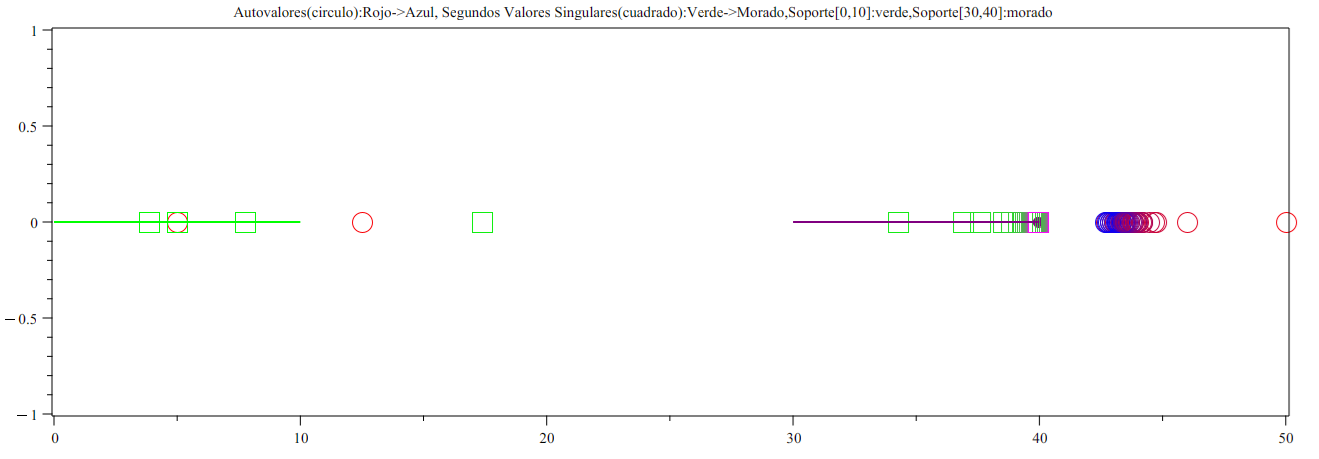
\includegraphics[width=\linewidth]{tfg_latex_etsiinf-2023.02.20/include/a0b10c30d40.png}
			\caption*{\scriptsize Sec. espectral}

		\end{subfigure}\hfill
		\begin{subfigure}[b]{0.4\columnwidth} % Modificado
			\tiny
			\textbf{Datos ($n=70$):}
			\begin{itemize}
				\item $\sigma_{1,70} \approx 9.27\text{e}16$
				\item $\sigma_{2,70} \approx 39.998$
				\item $R = 40$
				\item $\rho(\mathbf{D}_{70}) \approx 42.930$
				\item $\max\rho_k \approx 50.052$
			\end{itemize}
		\end{subfigure}
	\end{figure}
	\vspace{-1em}
\end{frame}

% --- DIAPOSITIVA 17A: CASO REAL - EJEMPLO ÁTOMO FUERA DEL SOPORTE ---
\begin{frame}{Caso Real: Átomo Fuera de $[-1,1]$}
	\textbf{Ejemplo 3:}\;
	$\displaystyle
		\langle p, q \rangle_S
		= \int_{-1}^{1} p(t) q(t) \, dt
		+ p'(2) q'(2)$
	\vspace{-0.8em}
	\begin{figure}
		\begin{subfigure}[b]{0.4\columnwidth} % Modificado
			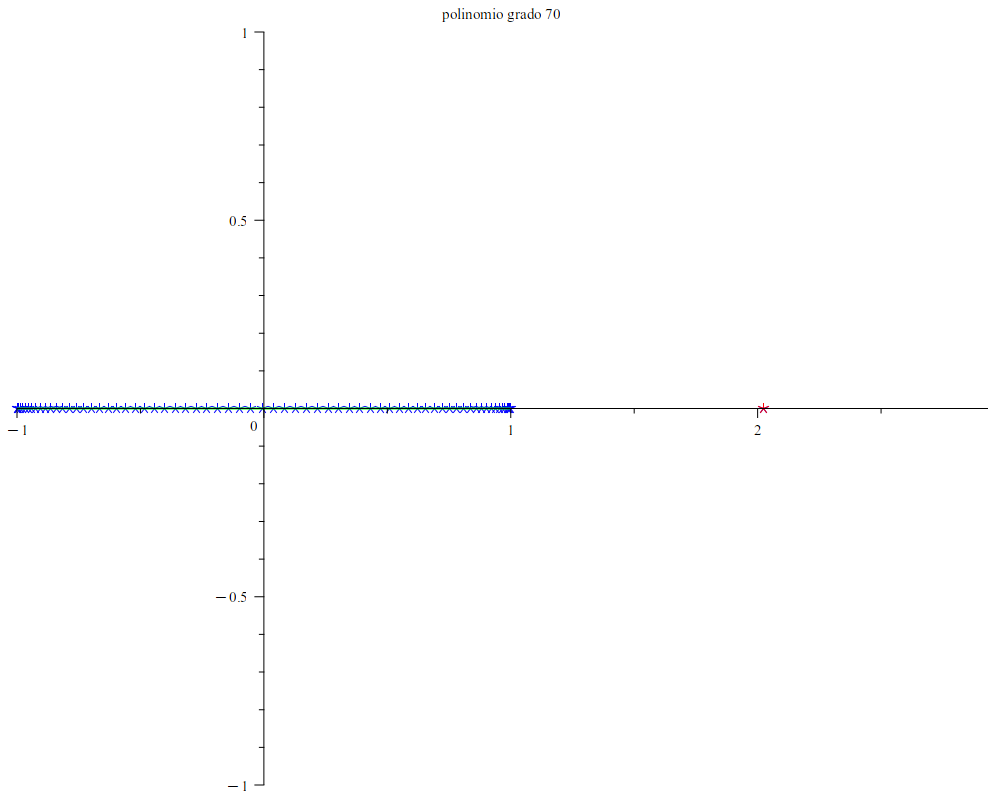
\includegraphics[width=\linewidth]{tfg_latex_etsiinf-2023.02.20/include/a-1b1t2_zero.png}
			\caption*{\scriptsize Ceros $\varphi_{70}$}
		\end{subfigure}\hfill
		\begin{subfigure}[b]{0.4\columnwidth} % Modificado
			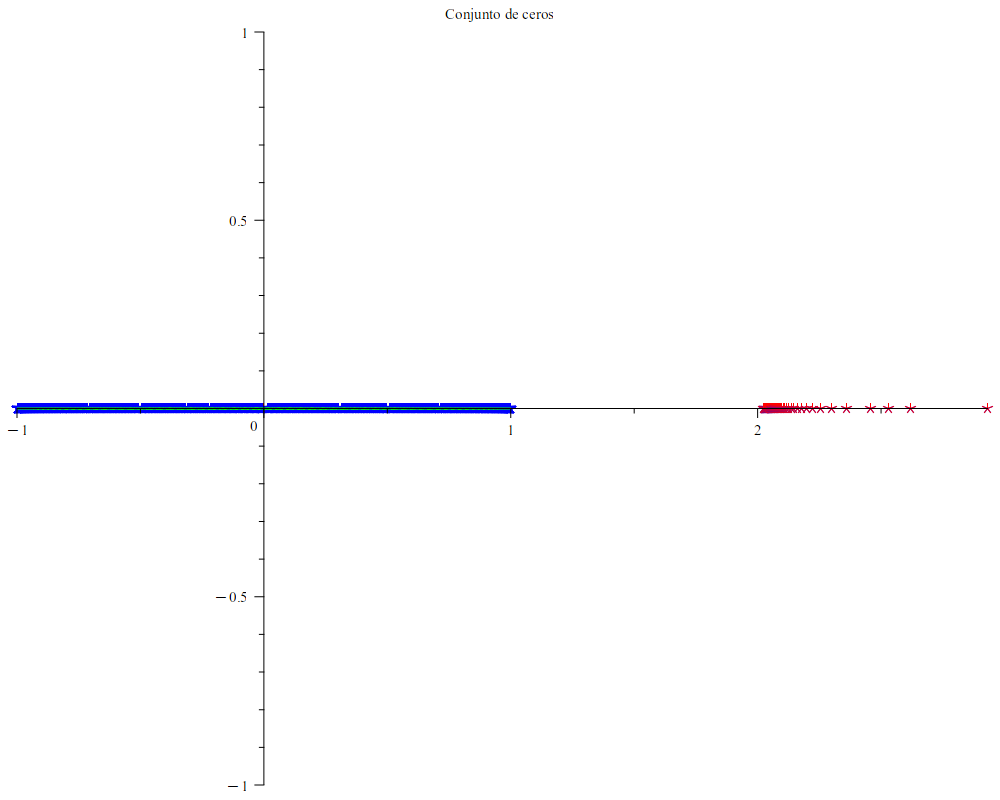
\includegraphics[width=\linewidth]{tfg_latex_etsiinf-2023.02.20/include/a-1b1t2_zeros.png}
			\caption*{\scriptsize Ceros $\varphi_{0},\dots,\varphi_{70}$}
		\end{subfigure}
		\vspace{-0.5em} % Modificado de -0.3em
		\begin{subfigure}[b]{0.4\columnwidth} % Modificado
			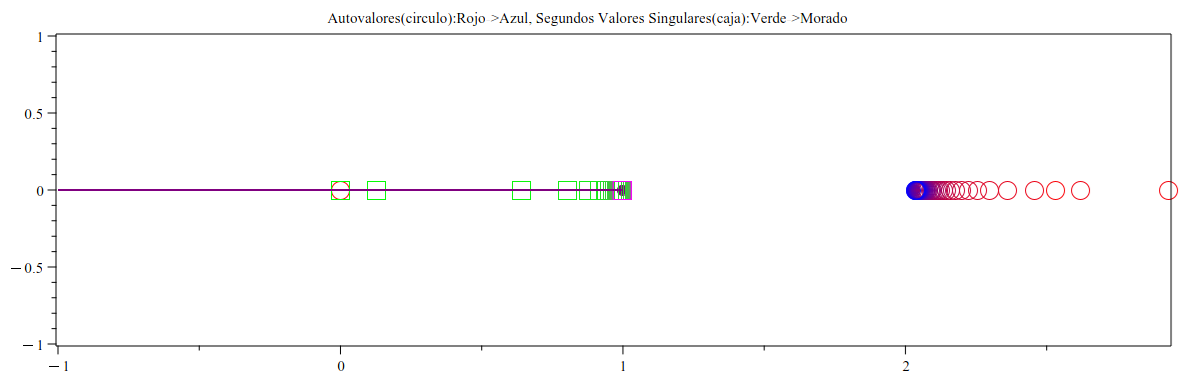
\includegraphics[width=\linewidth]{tfg_latex_etsiinf-2023.02.20/include/a-1b1t2.png}
			\caption*{\scriptsize Sec. espectral}
		\end{subfigure}\hfill
		\begin{subfigure}[b]{0.4\columnwidth} % Modificado
			\tiny
			\textbf{Datos ($n=70$):}
			\begin{itemize}
				\item $\sigma_{1,70} \approx 7.44\text{e}36$
				\item $\sigma_{2,70} \approx 0.999$
				\item $R = 2$ (átomo)
				\item $\rho(\mathbf{D}_{70}) \approx 2.025$
				\item $\max\rho_k \approx 2.933$
			\end{itemize}
		\end{subfigure}
	\end{figure}
	\vspace{-1em}
\end{frame}

% --- DIAPOSITIVA 17B: CASO REAL - EJEMPLO ÁTOMO FUERA (OBSERVACIONES) ---
\begin{frame}{Caso Real: Átomo Fuera de $[-1,1]$ - Observaciones}
	\begin{alertblock}{Observaciones (Ej.3)} \small
		Átomo $c=2$ fuera de $[-1,1]$. $\sigma_{1,n}$ diverge.
		$\rho(\mathbf{D}_n)$ acotado, influenciado por $c=2$.
		$\sigma_{2,n} \to \max_{[-1,1]}|z|=1$. Ceros atraídos por el átomo.
	\end{alertblock}
\end{frame}

% --- DIAPOSITIVA 18A: CASO CIRCUNFERENCIA - EJEMPLO SECUENCIALMENTE DOMINADO ---
\begin{frame}{Caso Circunferencia: Ejemplo Secuencialmente Dominado}
	\textbf{Ejemplo 4:}\;
	$\displaystyle
		\langle p, q \rangle_{S}=\int_{S_{1}(0)} p\overline{q}\, dm_{0;1} + \int_{S_{0.4}(0.4)} p'\overline{q'}\, dm_{0.4;0.4}$
	\vspace{-0.8em}
	\begin{figure}
		\begin{subfigure}[b]{0.4\columnwidth} % Modificado
			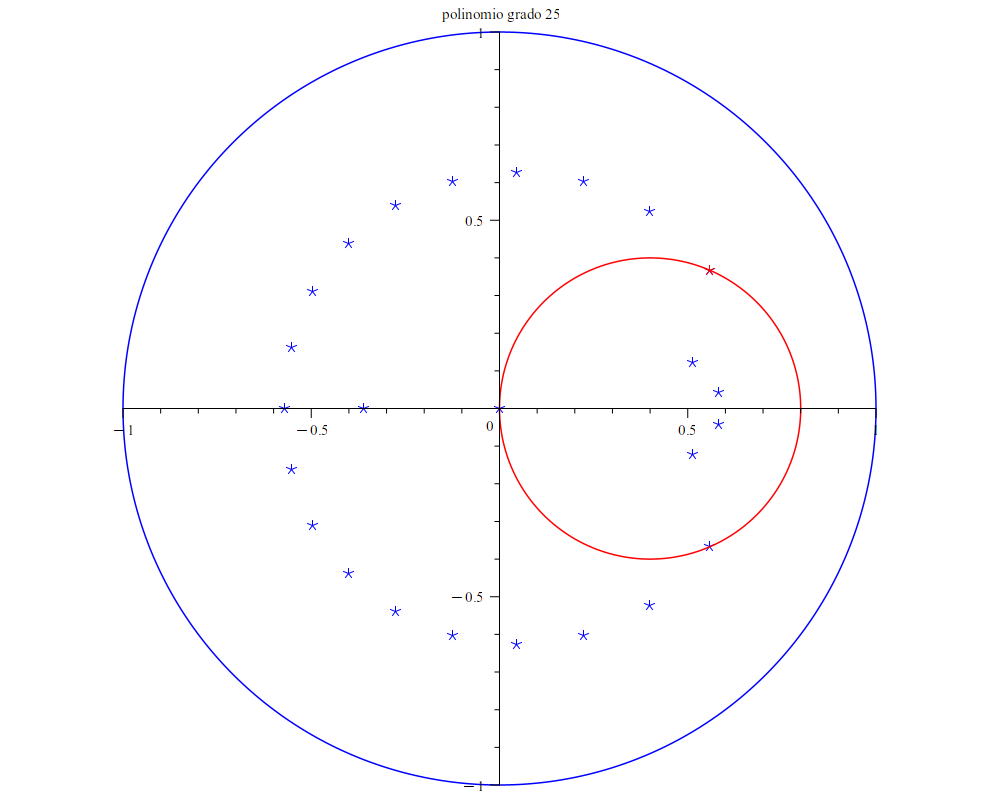
\includegraphics[width=\linewidth]{tfg_latex_etsiinf-2023.02.20/include/r1_1c1_0r2_0.4c2_0.4_zero.png}
			\caption*{\scriptsize Ceros $\varphi_{25}$}
		\end{subfigure}\hfill
		\begin{subfigure}[b]{0.4\columnwidth} % Modificado
			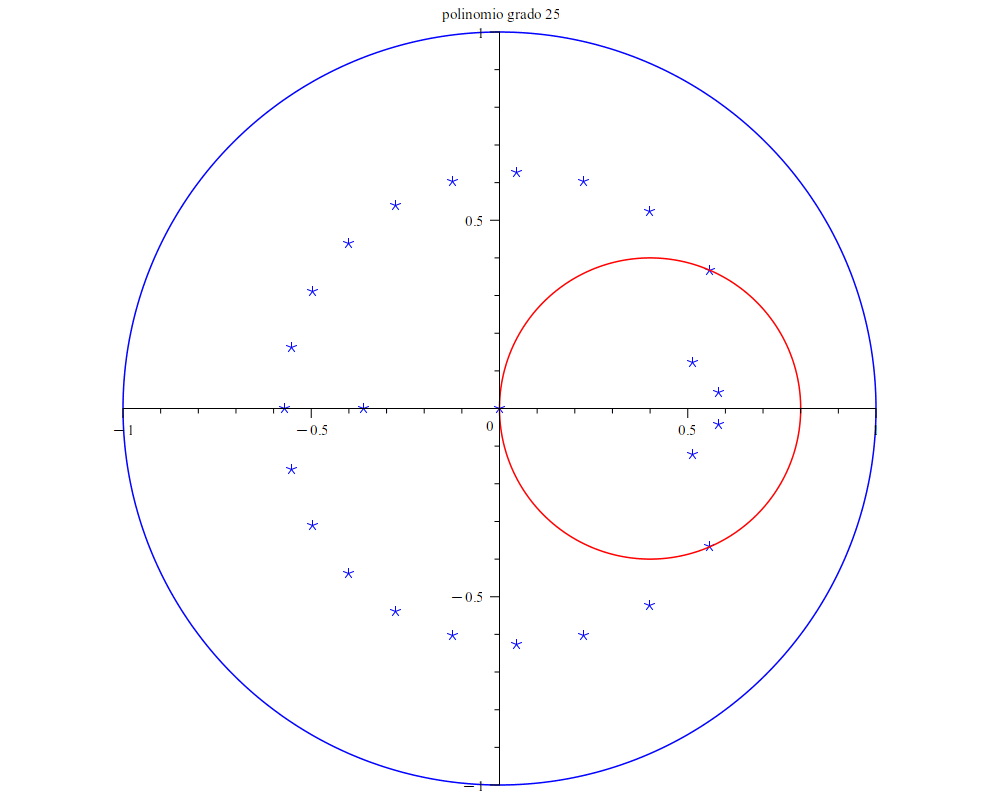
\includegraphics[width=\linewidth]{tfg_latex_etsiinf-2023.02.20/include/r1_1c1_0r2_0.4c2_0.4_zeros.png}
			\caption*{\scriptsize Ceros $\varphi_{0},\dots,\varphi_{25}$}
		\end{subfigure}
		\vspace{-0.5em} % Modificado de -0.3em
		\begin{subfigure}[b]{0.4\columnwidth} % Modificado
			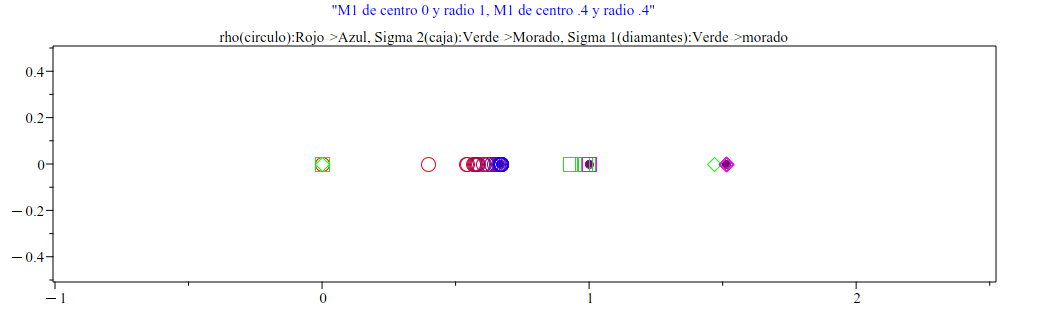
\includegraphics[width=\linewidth]{tfg_latex_etsiinf-2023.02.20/include/r1_1c1_0r2_0.4c2_0.4.png}
			\caption*{\scriptsize Sec. espectral}
		\end{subfigure}\hfill
		\begin{subfigure}[b]{0.4\columnwidth} % Modificado
			\tiny
			\textbf{Datos ($n=25$):}
			\begin{itemize}
				\item $\sigma_{1,25} \approx 1.516$
				\item $\sigma_{2,25} \approx 1.000$
				\item $R = 1$

				\item $\rho(\mathbf{D}_{25}) \approx 0.667$
				\item $\max\rho_k \approx 0.672$
			\end{itemize}
		\end{subfigure}
	\end{figure}
	\vspace{-1em}
\end{frame}

% --- DIAPOSITIVA 18B: CASO CIRCUNFERENCIA - EJEMPLO SEC. DOMINADO (OBSERVACIONES) ---
\begin{frame}{Caso Circunferencia: Ejemplo Secuencialmente Dominado - Observaciones}
	\begin{block}{Observaciones (Ej.4)} \small
		$S_{0.4}(0.4) \subset \mathbb{D}_1(0)$. $\mathcal{D}$ acotado. $\sigma_{1,n}$ converge.
		Ceros en $\mathbb{D}_1(0)$.
	\end{block}
\end{frame}

% --- DIAPOSITIVA 19A: CASO CIRCUNFERENCIA - EJEMPLO SOPORTES DISJUNTOS ---
\begin{frame}{Caso Circunferencia: Ejemplo Soportes Disjuntos}
	\textbf{Ejemplo 5:}\;
	$\displaystyle
		\langle p, q \rangle_{S}=\int_{S_{1}(0)} p\overline{q}\, dm_{0;1} + \int_{S_{1}(-10)} p'\overline{q'}\, dm_{-10;1}$
	\vspace{-0.8em}
	\begin{figure}
		\begin{subfigure}[b]{0.4\columnwidth} % Modificado
			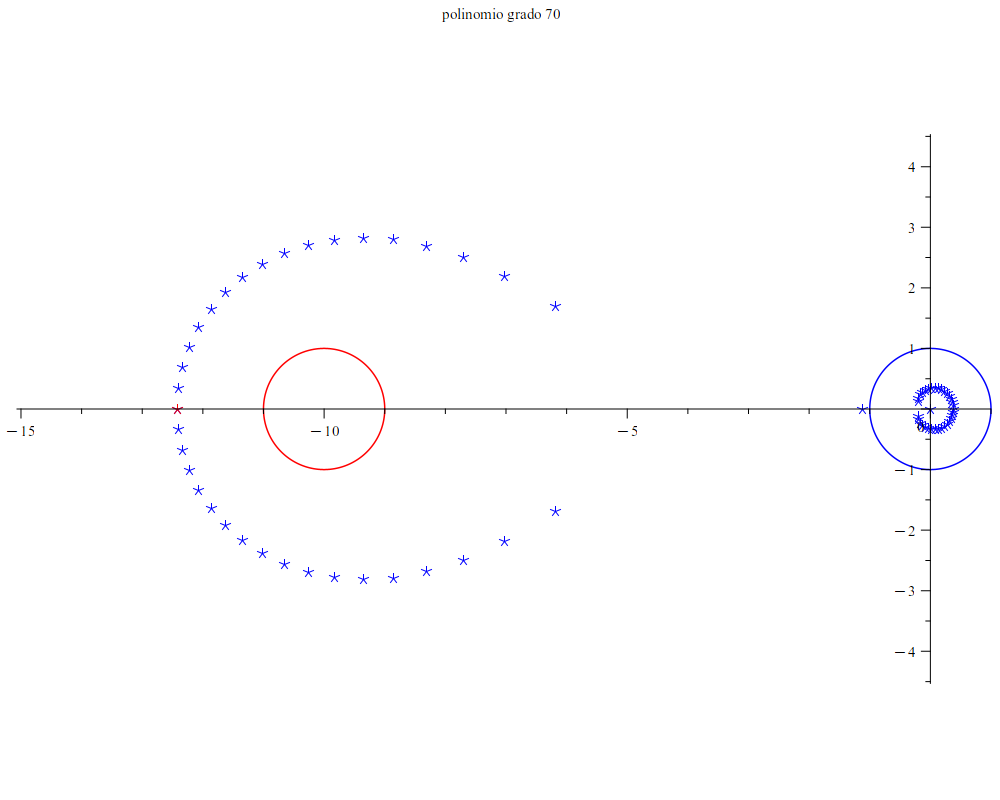
\includegraphics[width=\linewidth]{tfg_latex_etsiinf-2023.02.20/include/r1_1c1_0r2_1c2_-10_zero.png}
			\caption*{\scriptsize Ceros $\varphi_{70}$}
		\end{subfigure}\hfill
		\begin{subfigure}[b]{0.4\columnwidth} % Modificado
			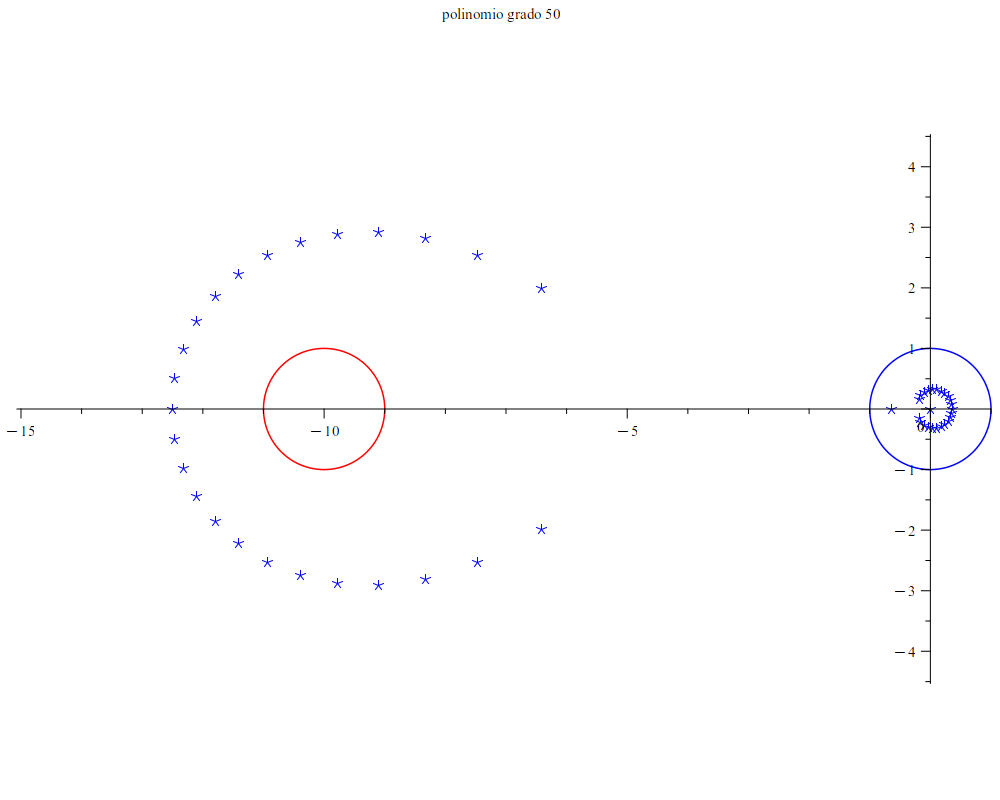
\includegraphics[width=\linewidth]{tfg_latex_etsiinf-2023.02.20/include/r1_1c1_0r2_1c2_-10_zeros.png}
			\caption*{\scriptsize Ceros $\varphi_{0},\dots,\varphi_{70}$}
		\end{subfigure}
		\vspace{-0.5em} % Modificado de -0.3em
		\begin{subfigure}[b]{0.4\columnwidth} % Modificado
			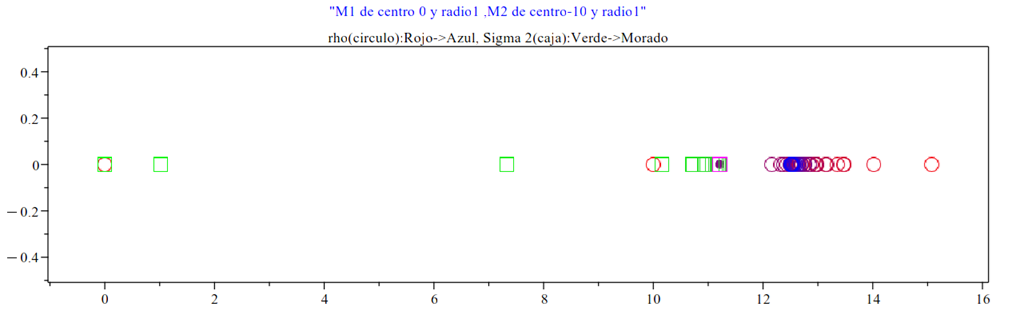
\includegraphics[width=\linewidth]{tfg_latex_etsiinf-2023.02.20/include/r1_1c1_0r2_1c2_-10.png}
			\caption*{\scriptsize Sec. espectral}
		\end{subfigure}\hfill
		\begin{subfigure}[b]{0.4\columnwidth} % Modificado
			\tiny
			\textbf{Datos ($n=70$):}
			\begin{itemize}
				\item $\sigma_{1,70} \approx 4.96\text{e}14$
				\item $\sigma_{2,70} \approx 11.211$
				\item $R = 11$
				\item $\rho(\mathbf{D}_{70}) \approx 12.424$
				\item $\max\rho_k \approx 15.074$
			\end{itemize}
		\end{subfigure}
	\end{figure}
	\vspace{-1em}
\end{frame}

% --- DIAPOSITIVA 19B: CASO CIRCUNFERENCIA - EJEMPLO SOP. DISJUNTOS (OBSERVACIONES) ---
\begin{frame}{Caso Circunferencia: Ejemplo Sop. Disjuntos - Observaciones}
	\begin{alertblock}{Observaciones (Ej.5)} \small
		Soportes disjuntos. $\sigma_{1,n}$ diverge.
		$\rho(\mathbf{D}_n)$ acotado. $\sigma_{2,n} \to R = 11$.
		Ceros pueden superar $R$.
	\end{alertblock}
\end{frame}

% --- DIAPOSITIVA 20A: CASO CIRCUNFERENCIA - EJEMPLO ÁTOMO FUERA ---
\begin{frame}{Caso Circunferencia: Ejemplo Átomo Fuera}
	\textbf{Ejemplo 6:}\;
	$\displaystyle
		\langle p, q \rangle_{S}=\int_{S_{1}(0)} p\overline{q}\, dm_{0;1} + p'(10)\overline{q'(10)}$
	\vspace{-0.8em}
	\begin{figure}
		\begin{subfigure}[b]{0.4\columnwidth} % Modificado
			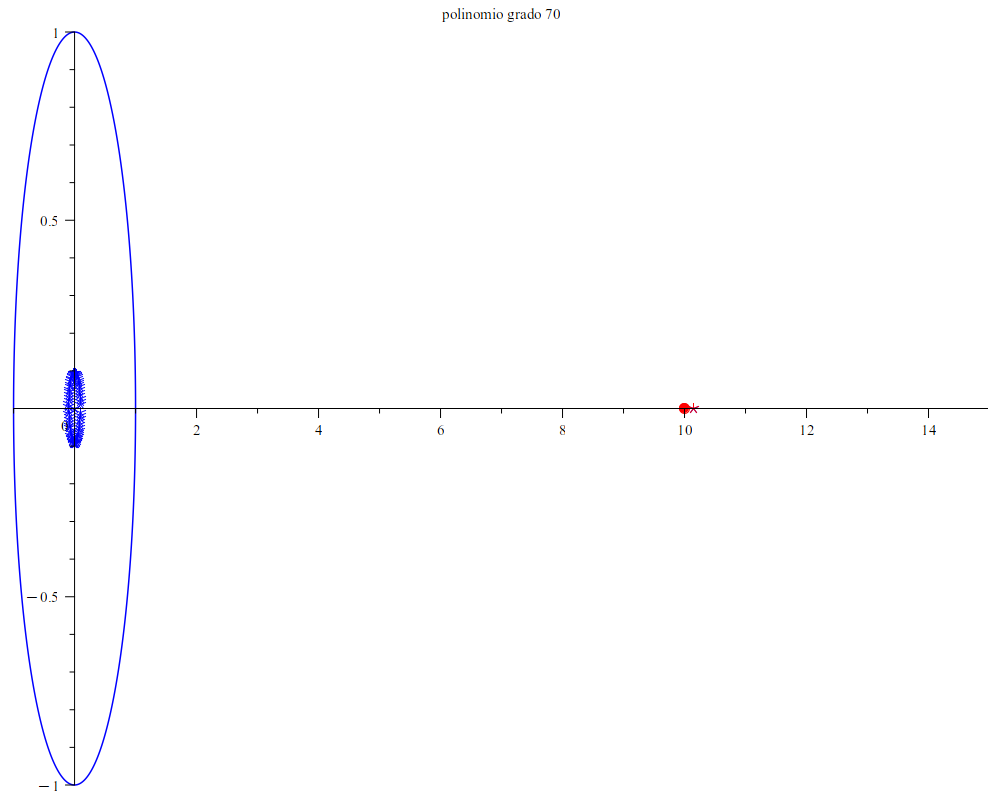
\includegraphics[width=\linewidth]{tfg_latex_etsiinf-2023.02.20/include/r1_1c1_0c2_10_zero.png}
			\caption*{\scriptsize Ceros $\varphi_{70}$}
		\end{subfigure}\hfill
		\begin{subfigure}[b]{0.4\columnwidth} % Modificado
			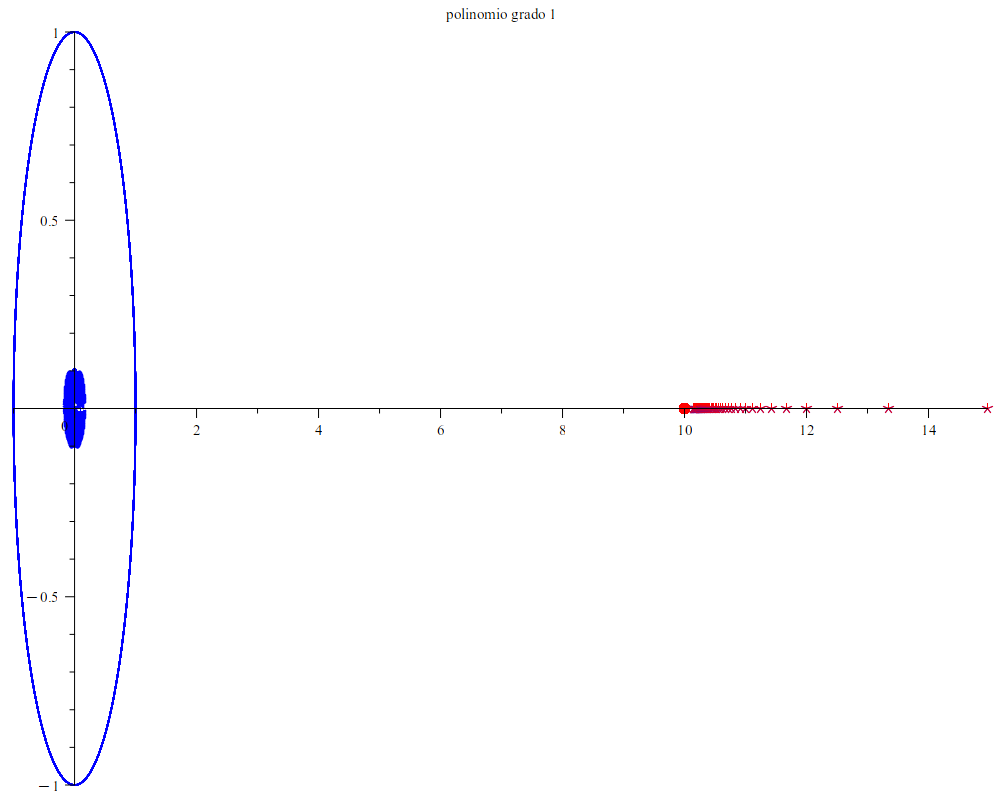
\includegraphics[width=\linewidth]{tfg_latex_etsiinf-2023.02.20/include/r1_1c1_0c2_10_zeros.png}
			\caption*{\scriptsize Ceros $\varphi_{0},\dots,\varphi_{70}$}
		\end{subfigure}
		\vspace{-0.5em} % Modificado de -0.3em
		\begin{subfigure}[b]{0.4\columnwidth} % Modificado
			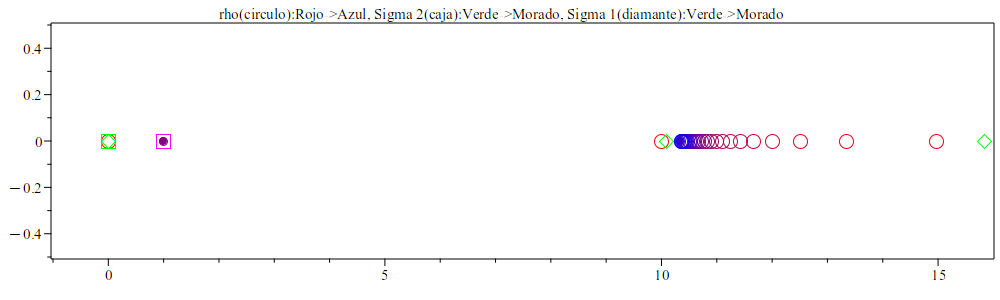
\includegraphics[width=\linewidth]{tfg_latex_etsiinf-2023.02.20/include/r1_1c1_0c2_10.png}
			\caption*{\scriptsize Sec. espectral}
		\end{subfigure}\hfill
		\begin{subfigure}[b]{0.4\columnwidth} % Modificado
			\tiny
			\textbf{Datos ($n=70$):}
			\begin{itemize}
				\item $\sigma_{1,70} \approx 3.50\text{e}26$
				\item $\sigma_{2,70} \approx 1.000$
				\item $R = 10$
				\item $\rho(\mathbf{D}_{70}) \approx 10.345$
				\item $\max\rho_k \approx 14.975$
			\end{itemize}
		\end{subfigure}
	\end{figure}
	\vspace{-1em}
\end{frame}

% --- DIAPOSITIVA 20B: CASO CIRCUNFERENCIA - EJEMPLO ÁTOMO FUERA (OBSERVACIONES) ---
\begin{frame}{Caso Circunferencia: Ejemplo Átomo Fuera - Observaciones}
	\begin{alertblock}{Observaciones (Ej.6)} \small
		Átomo $c=10$ fuera de $\mathbb{D}_1(0)$. $\sigma_{1,n}$ diverge.
		$\rho(\mathbf{D}_n)$ acotado, influenciado por $c=10$.
		$\sigma_{2,n} \to 1$. Ceros atraídos por el átomo.
	\end{alertblock}
\end{frame}

% --- DIAPOSITIVA 21A.1: ANÁLISIS Y CONJETURAS (IA) - OBSERVACIONES (SEC. DOMINADO) ---
\begin{frame}{Análisis y Conjeturas (Ia): Observaciones (Sec. Dominado)}
	\begin{block}{Caso Secuencialmente Dominado (Continuo Real)} \small
		El Cuadro 3.1 revela que en ejemplos secuencialmente dominados (e.g., Ej.1), donde $I_2=[c,d] \subset I_1=[a,b]$ y $w_1(t)/w_0(t)$ acotado en $I_1$:
		\begin{itemize}
			\item El operador multiplicación $\mathcal{D}$ es acotado.
			\item Los valores singulares $\sigma_{1,n}, \sigma_{2,n}$ y $\rho(\mathbf{D}_n)$ confirman la acotación.
			\item Los ceros están acotados por $\|\mathcal{D}\|$.
		\end{itemize}
	\end{block}
	\pause
	\begin{block}{Proposición (Caso Continuo Real)} \small
		Para $I_1=[a,b]$, $I_2=[c,d]$ con $[c,d] \subset [a,b]$, si definimos:
		$$R = \max\{|a|,|b|,|c|,|d|\}, \quad \alpha = \max_{t\in[a,b]}\frac{w_1(t)}{w_0(t)}$$
		Entonces $\mathcal{D}$ es acotado y $\|\mathcal{D}\| \le \sqrt{2(R^{2}+\alpha)}$.
	\end{block}
\end{frame}

% --- NUEVA DIAPOSITIVA: DEMOSTRACIÓN DE LA PROPOSICIÓN ---
\begin{frame}{Demostración: Operador Acotado (Caso Secuencialmente Dominado)}
	\begin{block}{Demostración} \tiny
		Sea $p(t)\in\mathbb{P}[t]$. Utilizando que $(a+b)^2\leq 2(a^2+b^2)$ para $a,b\ge0$:
		\begin{align}
			\|\mathcal{D}(p(t))\|^{2} & = \int_{a}^{b} t^2 p^2(t) w_0(t)\,dt + \int_{c}^{d} [(tp(t))']^2 w_1(t)\,dt                                            \\
			                          & = \int_{a}^{b} t^2 p^2(t) w_0(t)\,dt + \int_{c}^{d} [p(t)+tp'(t)]^2 w_1(t)\,dt                                         \\
			                          & \le \int_{a}^{b} t^2p^2(t)w_0(t)\, dt+2\left(\int_{c}^{d} p(t)^2w_1(t)\, dt +\int_{c}^{d} t^2p'(t)^2w_1(t)\, dt\right)
		\end{align}
	\end{block}
\end{frame}

% --- CONTINUACIÓN DE LA DEMOSTRACIÓN ---
\begin{frame}{Demostración: Operador Acotado (Continuación)}
	\begin{block}{Demostración (Continuación)} \tiny
		\begin{align}
			 & \le R^{2} \left(\int_{a}^{b} p^2(t)w_0(t)\, dt +  2\int_{c}^{d} p'(t)^2w_1(t)\, dt\right)+ 2\int_{c}^{d} p(t)^2w_1(t)\, dt \\
			 & \le 2R^{2} \|p(t)\|^{2} + 2\alpha \int_{c}^{d} p(t)^2w_0(t)\, dt                                                           \\
			 & \le 2R^{2} \|p(t)\|^{2} + 2\alpha \int_{a}^{b} p(t)^2w_0(t)\, dt                                                           \\
			 & = 2(R^{2}+\alpha)\|p(t)\|^{2}
		\end{align}
		Por tanto, $\|\mathcal{D}\| \le \sqrt{2(R^{2}+\alpha)}$. \qed
	\end{block}

	\begin{exampleblock}{Aplicación a los Ejemplos} \tiny
		\textbf{Ejemplo 1:} $I_1 = [-1,1]$ (con $w_0(t)=t^2$), $I_2 = [-1,1]$ (con $w_1(t)=t^{10}$).
		$R = 1$, $\alpha = 1$, entonces $\|\mathcal{D}\| \le \sqrt{4} = 2$.
		Consistente con $\sigma_{1,70} = 1.276 \le 2$.

		\textbf{Ejemplo 2:} $I_1 = [-2,2]$, $I_2 = [-1,1]$.
		$R = 2$, $\alpha = 1$, entonces $\|\mathcal{D}\| \le \sqrt{10} \approx 3.16$.
		Consistente con $\sigma_{1,70} = 1.999$.
	\end{exampleblock}
\end{frame}

% --- DIAPOSITIVA: CASOS NO SECUENCIALMENTE DOMINADOS ---
\begin{frame}{Análisis: Casos No Secuencialmente Dominados}
	\begin{alertblock}{Observaciones (Ejemplos 4-11)} \small
		Para casos con soportes disjuntos ($I_1 \cap I_2 = \emptyset$):
		\begin{itemize}
			\item $\sigma_{1,n}$ crece exponencialmente ($\approx 10^{16}$), sugiriendo $\mathcal{D}$ no acotado.
			\item $\sigma_{2,n}$ converge a $R = \max\{|a|,|b|,|c|,|d|\}$.
			\item $\rho(\mathbf{D}_n)$ permanece acotado, con comportamiento dependiente de la geometría:
			      \begin{itemize}
				      \item Si $I_1$ contiene el extremo de mayor módulo: $\rho(\mathbf{D}_n) \to R$.
				      \item Si $I_2$ contiene el extremo de mayor módulo: $\rho(\mathbf{D}_n) \to R + k$ con $k \geq 0$.
			      \end{itemize}
		\end{itemize}
	\end{alertblock}
\end{frame}

% --- DIAPOSITIVA: CASOS CON ÁTOMO ---
\begin{frame}{Análisis: Casos con Átomo}
	\begin{alertblock}{Observaciones (Ejemplos 12-15)} \small
		Para productos $\langle p,q \rangle = \int_{a}^{b} pq \, dt + p'(c)q'(c)$:
		\begin{itemize}
			\item $\sigma_{1,n}$ extremadamente grande ($\approx 10^{36}$), indicando $\mathcal{D}$ no acotado.
			\item $\sigma_{2,n}$ converge a $R_0 = \max\{|a|,|b|\}$ (radio del soporte integral).
			\item Comportamiento de $\rho(\mathbf{D}_n)$ depende de la posición del átomo:
			      \begin{itemize}
				      \item Si $c \in [a,b]$: $\rho(\mathbf{D}_n) \to R_0$.
				      \item Si $c \notin [a,b]$: $\rho(\mathbf{D}_n)$ influenciado por $|c|$, ceros atraídos hacia $c$.
			      \end{itemize}
		\end{itemize}
	\end{alertblock}
\end{frame}

% --- DIAPOSITIVA: CASO CIRCUNFERENCIA - ANÁLISIS ---
\begin{frame}{Análisis: Caso Circunferencia}
	\begin{block}{Clasificación por Contención} \small
		Para productos $\langle p,q \rangle = \int_{S_{r_b}(b)} p\overline{q} \, dm + \int_{S_{r_a}(a)} p'\overline{q'} \, dm$:
		\begin{enumerate}
			\item \textbf{$S_{r_a}(a) \subset \mathbb{D}_{r_b}(b)$}: Caso secuencialmente dominado, $\mathcal{D}$ acotado.
			\item \textbf{$a \in \mathbb{D}_{r_b}(b)$ pero $S_{r_a}(a) \not\subset \mathbb{D}_{r_b}(b)$}: $\mathcal{D}$ acotado.
			\item \textbf{$a \notin \mathbb{D}_{r_b}(b)$}: Comportamiento de $\mathcal{D}$ incierto, evidencia sugiere no acotación.
		\end{enumerate}
	\end{block}
	\pause
	\begin{block}{Casos con Átomo Complejo} \small
		\begin{itemize}
			\item Si $c \in \mathbb{D}_{r_b}(b)$: $\mathcal{D}$ acotado (casos secuencialmente dominados).
			\item Si $c \notin \mathbb{D}_{r_b}(b)$: Evidencia sugiere $\mathcal{D}$ no acotado.
		\end{itemize}
	\end{block}
\end{frame}

% --- DIAPOSITIVA 21B: ANÁLISIS Y CONJETURAS (IB) - OBSERVACIONES CLAVE ---
\begin{frame}{Análisis y Conjeturas (Ib): Observación Fundamental}
	\begin{alertblock}{Observación Crucial (Todos los Ejemplos)} \small
		En la totalidad de los ejemplos numéricos (Cuadros 3.1 y 3.2):
		\begin{itemize}
			\item \textbf{Acotación Universal del Radio Espectral}: Incluso cuando $\mathcal{D}$ no es acotado ($\sigma_{1,n} \to \infty$), el radio espectral $\rho(\mathbf{D}_n)$ permanece acotado.
			\item \textbf{Convergencia del Segundo Valor Singular}: $\sigma_{2,n}$ converge consistentemente:
			      \begin{itemize}
				      \item En casos continuos: a $R = \max\{|z| : z \in \text{supp}(\mu_1) \cup \text{supp}(\mu_2)\}$.
				      \item En casos con átomo: a $R_0 = \max\{|z| : z \in \text{supp}(\mu_1)\}$.
			      \end{itemize}
		\end{itemize}
	\end{alertblock}
\end{frame}

% --- DIAPOSITIVA: SOPORTE TEÓRICO ---
\begin{frame}{Soporte Teórico: Teoremas de Entrelazamiento}
	\begin{block}{Teorema de Entrelazamiento de Cauchy} \small
		Sea $A$ matriz de orden $n$ y $B$ submatriz principal de orden $n-1$. Si $\lambda_n \leq \cdots \leq \lambda_1$ son autovalores de $A$ y $\mu_{n-1} \leq \cdots \leq \mu_1$ de $B$:
		$$\lambda_n \leq \mu_{n-1} \leq \cdots \leq \mu_2 \leq \lambda_1$$
	\end{block}
	\pause
	\begin{block}{Aplicación a Matrices de Hessenberg} \small
		Para matrices infinitas de Hessenberg $\mathbf{D}$ con secciones $\mathbf{D}_n$:
		\begin{itemize}
			\item La sucesión $\{\sigma_{2,n}\}$ es creciente.
			\item Existe $\lim_{n \to \infty} \sigma_{2,n} \leq \infty$.
		\end{itemize}
	\end{block}
\end{frame}

% --- DIAPOSITIVA 22A.1: CONJETURAS PRINCIPALES (IIA) - CONJETURA 1 (ACOTACIÓN) ---
\begin{frame}{Conjetura 1: Acotación Universal del Radio Espectral}
	\begin{block}{Conjetura Principal} \small
		Basándose en la evidencia numérica exhaustiva de los Cuadros 3.1 y 3.2:
		$$\lim_{n \to \infty} \rho(\mathbf{D}_n) < \infty$$
		Esta propiedad se mantiene incluso cuando el operador $\mathcal{D}$ no es acotado.
	\end{block}
	\pause
	\begin{block}{Comportamiento Asintótico} \small
		El radio espectral tiende a converger a $R + k$, donde:
		\begin{itemize}
			\item $R = \max\{|z| : z \in \text{supp}(\mu_1) \cup \text{supp}(\mu_2)\}$
			\item $k \in \mathbb{R}$ depende de la geometría relativa de los soportes
			\item $k \geq 0$ cuando el soporte de la derivada contiene el extremo de mayor módulo
		\end{itemize}
	\end{block}
\end{frame}

% --- DIAPOSITIVA 22b: CONJETURAS PRINCIPALES (IIIB) - FORMULACIÓN ---
\begin{frame}{Conjetura 2: Convergencia del Segundo Valor Singular}
	\begin{block}{Conjetura 2} \small
		El segundo mayor valor singular $\sigma_{2,n}$ de $\mathbf{D}_n$ converge:
		$$\lim_{n \to \infty} \sigma_{2,n} < \infty$$
		Específicamente:
		\begin{itemize}
			\item En casos continuos: converge a $R = \max\{|z| : z \in \text{supp}(\mu_1) \cup \text{supp}(\mu_2)\}$
			\item En casos con átomo: converge a $R_0 = \max\{|z| : z \in \text{supp}(\mu_1)\}$
		\end{itemize}
	\end{block}
	\pause
	\begin{exampleblock}{Soporte Teórico} \small
		Resultados parciales apoyan estas conjeturas:
		\begin{itemize}
			\item Teorema de entrelazamiento de Cauchy
			\item Propiedades de matrices de Hessenberg
			\item Análisis de valores singulares \cite{singularValuesOfHessenbergMatrices}
		\end{itemize}
	\end{exampleblock}
\end{frame}

% --- DIAPOSITIVA 23A.1: ANÁLISIS Y CONJETURAS (IIIA) - TRASLACIONES (OBSERVACIÓN Y CONJETURA) ---
\begin{frame}{Conjetura 3: Traslaciones de Soportes}
	\begin{block}{Observación Empírica} \small
		Cuando los soportes en $\mathbb{R}$ se trasladan a lo largo del eje real, los ceros se trasladan de manera correspondiente.
	\end{block}
	\pause
	\begin{block}{Conjetura 3} \small
		Los ceros de polinomios ortogonales de Sobolev asociados a medidas trasladadas en el eje real se trasladan mediante la misma traslación.
	\end{block}
	\pause
	\begin{alertblock}{Limitaciones} \small
		Si la traslación tiene componente imaginaria, pueden ocurrir comportamientos anómalos que requieren investigación adicional.
	\end{alertblock}
\end{frame}

% --- DIAPOSITIVA 23B: ANÁLISIS Y CONJETURAS (IIIB) - SEMEJANZA ---
\begin{frame}{Transformaciones de Semejanza: Limitaciones en Sobolev}
	\begin{block}{Caso Estándar (Una Medida)} \small
		Si $f(z) = \alpha z + \beta$ es una semejanza, los ceros de $P_n(z)$ se transforman mediante $f$ a los ceros de $P_n^f(z)$.
	\end{block}
	\pause
	\begin{alertblock}{Precaución en Productos de Sobolev} \small
		En productos de Sobolev, la aplicabilidad directa de este resultado \textbf{no es general}:
		\begin{itemize}
			\item Ejemplos con traslaciones complejas muestran comportamientos anómalos
			\item La teoría clásica de transformaciones no se extiende automáticamente
			\item Se requiere investigación específica para productos de Sobolev
		\end{itemize}
	\end{alertblock}
\end{frame}

% --- DIAPOSITIVA FINAL: RESUMEN DE CONJETURAS ---
\begin{frame}{Resumen: Conjeturas Principales}
	\begin{block}{Tres Conjeturas Fundamentales} \small
		\begin{enumerate}
			\item \textbf{Acotación Universal}: $\lim_{n \to \infty} \rho(\mathbf{D}_n) < \infty$ incluso cuando $\mathcal{D}$ no es acotado.
			\item \textbf{Convergencia $\sigma_2$}: $\lim_{n \to \infty} \sigma_{2,n} = R$ (casos continuos) o $R_0$ (casos atómicos).
			\item \textbf{Invarianza por Traslación}: Los ceros se trasladan con traslaciones reales de los soportes.
		\end{enumerate}
	\end{block}
	\pause
	\begin{exampleblock}{Implicaciones} \small
		Estas conjeturas establecen:
		\begin{itemize}
			\item Cotas universales para ceros de polinomios de Sobolev
			\item Criterios predictivos basados en la geometría de soportes
			\item Fundamentos para futuras demostraciones rigurosas
		\end{itemize}
	\end{exampleblock}
\end{frame}